\chapter{Analysis of existing company}

As an example of an existing service implementation let's take an anonymous international company. For the purpose of this thesis it will be named Invest s.r.o.. It operates in finantial sector and provides a platform for investment companies. Invest s.r.o. already exists more than ten years and during this period was reorganised to service-oriented architecture. The company has many clients in its portfolio. Many of them are consuming services provided by this company.

\section{Architecture overview}
Architecture of Invest s.r.o. can be divided into multiple layers. In sake of providing services to the third party the application is composed by Data layer, Application layer, Integration layer as is shown on Figure \ref{fig:invest-architecture}.

\begin{figure}[htp] \centering{
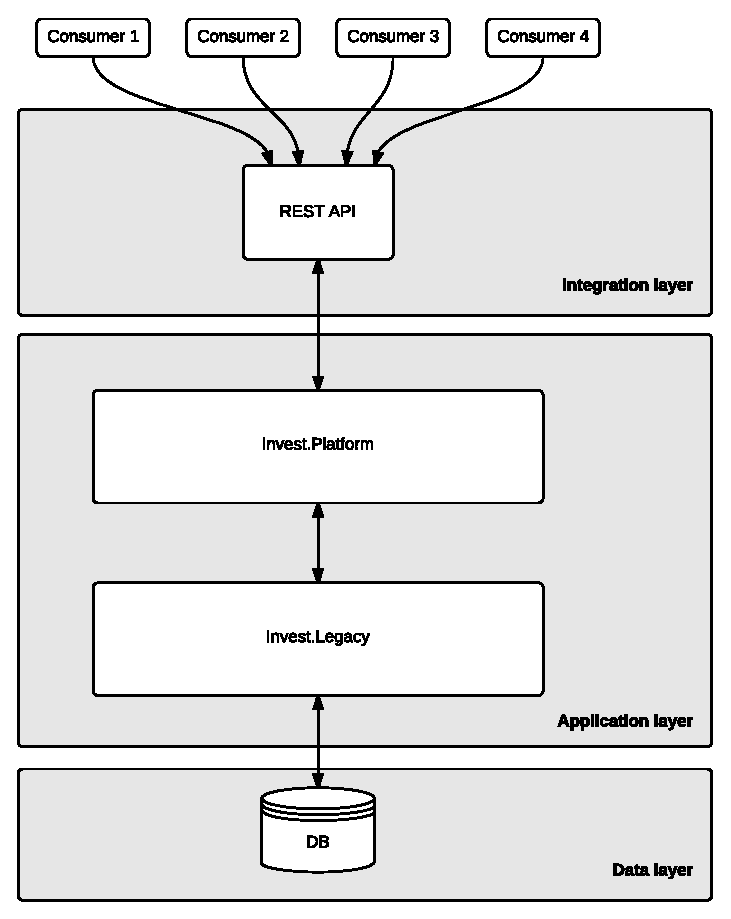
\includegraphics[width=8cm]{img/invest-architecture.pdf}}
\caption{Invest s.r.o. architecture}
\label{fig:invest-architecture}
\end{figure} 

The highest layer of application is Integration layer containing service API. It provides access points to underlying logic. Services consumers integrate it to their applicaton. The Application layer holds the whole business logic. Every logical functionality is performed in this layer. Data layer is accessed by \gls{dal} components, it contains various data stores.

\section{Integration layer}
Services of Invest s.r.o. are REST-based. The HTTP methods are used for communication between the company and its clients. A service is accessed by URL template and HTTP verbs such as GET, POST, PUT and DELETE. For example, to retrieve a bank account with concrete id the service call looks like: 

\begin{lstlisting}
    GET    /api/v3/bankaccounts/{bankAccountId}
\end{lstlisting}

In service request the \emph{\{bankAccountId\}} part of URL is replaced by bank account identifier which the client wants to obtain in response.

HTTP messages can be sent in XML or JSON format. Services are able to process both of them. Headers like Content-type and Accept can be filled by one of them:
 
\begin{lstlisting}
    Content-type: application/json
    Accept: application/json
\end{lstlisting}

Invest s.r.o service API contains many services. Their capabilities and usage is part of an available \gls{documentation}. Client can take set of services to compose a business processes. 

As an example, client has a login process through which an user passes to access his user account. User has to provide the user name, user password and memorable word. After filling them correctly the user can operate with his account. The business process is composed form these requests:

\begin{lstlisting}
    POST /api/v3/session
    POST /api/v3/memorablewords
\end{lstlisting}
  
To log-in into the account client sends two request to the server (Figure \ref{fig:login-process}). The first of them authenticates the credentials and starts the \gls{session}. The other one make another identity check. It posts the user's answer on asked memorable word characters. When both requests return successful response (200 OK), the user is logged in to his account otherwise the access is denied.

\begin{figure}[htp] \centering{
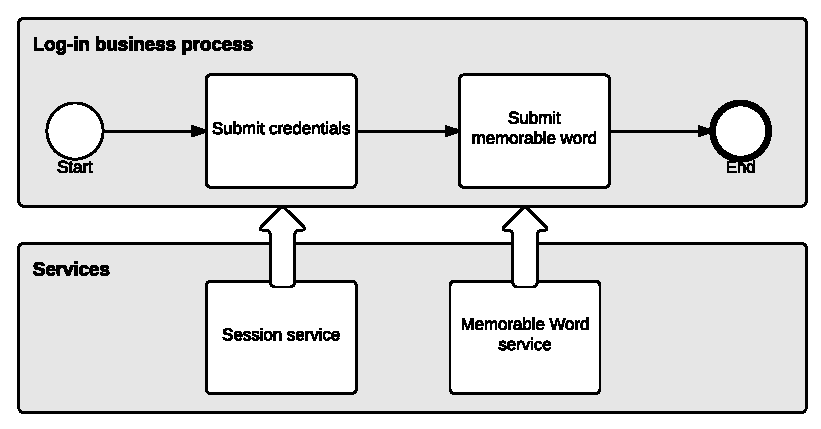
\includegraphics[width=8cm]{img/login-process.pdf}}
\caption{Log-in process and particular services calls}
\label{fig:login-process}
\end{figure} 


\section{Developmnet and deployment}
The company uses an \gls{scm} (SCM) to track the changes made in service implementation during the development phase. There is a master version of API to which are promoted the changes from multiple developers. The implementation is then built by Continuous Integration tool. 

The CI automaticaly increases the version of implementation after every successful build. The new version's DLL file is deployed on the environment. 

There are more than one version of API developed at the same time. The concrete version is maintained until it has a client which uses it. Parallel development means that bugs have to be fixed in every used version. Thanks to SCM it is possible to transfer a fix accross the versions which contains the error. 

\subsection{Environments}
The Invest s.r.o uses many environments to develop, test, simulate usage and provide the API. On Figure \ref{fig:environments-hierarchy} is an example of the environment hierarchy on which the API version is deployed before is deployed in production.

\begin{figure}[htp] \centering{
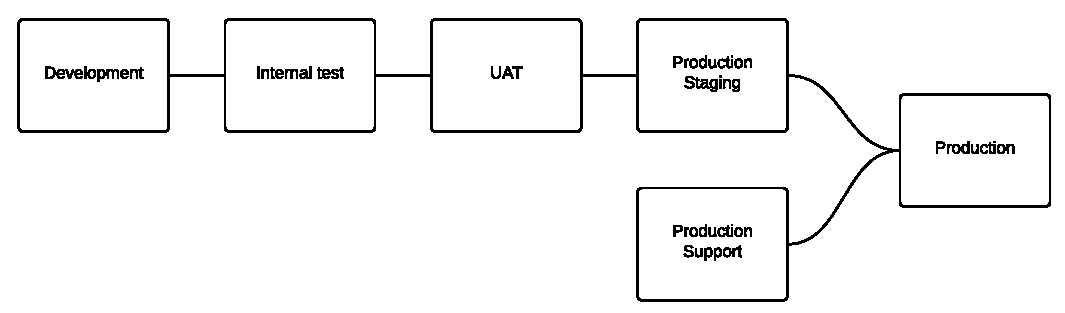
\includegraphics[width=12cm]{img/environments-hierarchy.pdf}}
\caption{Environments hierarchy}
\label{fig:environments-hierarchy}
\end{figure} 

Development environment serves for development. Internal test environment is for functional testing. On \gls{uat} environment users tests whether the application handle all real-world scenarios according to specification. Staging environment take a part before the production release. It serves to discover eventual errors before the deployment into production. Production environment is used by client. Production support is environment synchronized with Production one, it provides the possibility to support the API which is already in use.

Every API version has its hierarchy of environments on which is developed and tested. Every client has its own production environment with one deployed version of API. When client wants to switch to the different version, it has to be deployed replacing the old one.


\section{Versioning of services}
The Invest s.r.o. deals with many change requests within the provided application. The company has to adapt the application functionality to the newest legislative rules deriving from financial authorities. Other adjustment requests are asked by clients. The change requests can result in modifications of services.

\subsection{Versioning strategy}
The strategy of Invest s.r.o is based on avoiding the breaking changes. The company is trying to transform every change in compatible one. A new version of service interface doesn't break the usage of API by the clients. The company has a \emph{flexible strategy} to versioning the services. The comptible changes don't cause the creation of a new version.
The API in fact has its version. The new API version is created when it is convenient for functionality of API.
 

\subsection{Version lifecycle}
The version of Invest.API is created after a period of time and certain amount of changes, other reason can be a necessity to make a breaking change. Every modification of service interface is on implementation level. These changes cause that the code is slowly becoming big and harder to maintain. In cerain moment the Invest s.r.o. can deside to create a new version of API. API version contains cleaned code and its number increases.  Duration of version lifecycle in the company is in the range of years. 
 
\subsection{API version in URL}
The company is versioning whole service API, not only services or service methods. The approach to versioning is the one which is used to version software in general. When a new version is created and deployed to production environment the old version is no longer accessible. It can be said that the version number in URL is informative. It suggests to clients that they have to call requests according to \gls{documentation} of this API version. Current API version of Invest s.r.o has the version \emph{v3}. For example, let's have a Customers service in Invest.API. The URL to post action than looks like:

\begin{lstlisting}
  POST   \api\v3\customers
\end{lstlisting}

The version in URL can't be changed because the API doesn't have other accessible version. The URL is stable. Eventual changes in Customer service are always backward compatible and wouldn't influence the consumers. 

\subsection{Service interface changes}
When it is needed to change a service interface, the company tries to don't affect any of its clients. For example after a change in implementation of service one of the elements of representation doesn't hold enough information anymore. There is a need to encapsulate this element into another one. Let's have bank account which representation contains mandatory elements. The request is:

\begin{lstlisting}
  <?xml version="1.0"?>
  <BankAccount>
    <BankAccountId>1</BankAccountId>
    <BankAccountNumber>12345678</BankAccountNumber>
    <BankName>InvestBank</BankName>
    <BankAccountName>MyBankAccount</BankAccountName>
  </BankAccount>
\end{lstlisting}

After a change of the requirements there is a need to have \emph{BankAddress} element in representation. \emph{BankAddress} and \emph{BankName} will be encapsulated into the node \emph{bankDetails}. The new request then should look like:

\begin{lstlisting}
  <?xml version="1.0"?>
  <BankAccount>
    <BankAccountId>1</BankAccountId>
    <BankAccountNumber>12345678</BankAccountNumber>
    <BankDetails>
      <BankName>InvestBank</BankName>
      <BankAddress>
        <Line1>Road 12</Line1>
        <Line2>London</Line2>
        <PostCode>AA0000A</PostCode>
      </BankAddress>
    </BankDetails>
    <BankAccountName>MyBankAccount</BankAccountName>
  </BankAccount>
\end{lstlisting}

If the change will be deployed it will harm the usability of application for each client who expects the old version. It is a breaking change which would force all clients to integrate this change or the provider to create a new version of a service. The Invest s.r.o. doesn't want to change the service interface but adds a new feature. The new representation contains new elemenet with the encapsulation and at the same time the old element which is marked as obsolete.

\begin{lstlisting}
  <?xml version="1.0"?>
  <BankAccount>
    <BankAccountId>1</BankAccountId>
    <BankAccountNumber>sample string</BankAccountNumber>
    <BankName>sample string</BankName>                      (obsolete element)
    <BankDetails>
      <BankName>sample string</BankName>
      <BankAddress>
        <Line1>sample string</Line1>
        <Line2>sample string</Line2>
        <PostCode>sample string</PostCode>
      </BankAddress>
    </BankDetails>
    <BankAccountName>sample string</BankAccountName>
  </BankAccount>
\end{lstlisting}

Both elements have to be optional because clients make calls just with one of them. In service implementation the code for both kinds of received data has to be present. The situation when one client sends a request with obsolete element \emph{BankName} and the other one with the new element \emph{BankDetails} is shown on Figure \ref{fig:compatible-api-change}. Both requests are valid BankAccounts service calls.

\begin{figure}[htp] \centering{
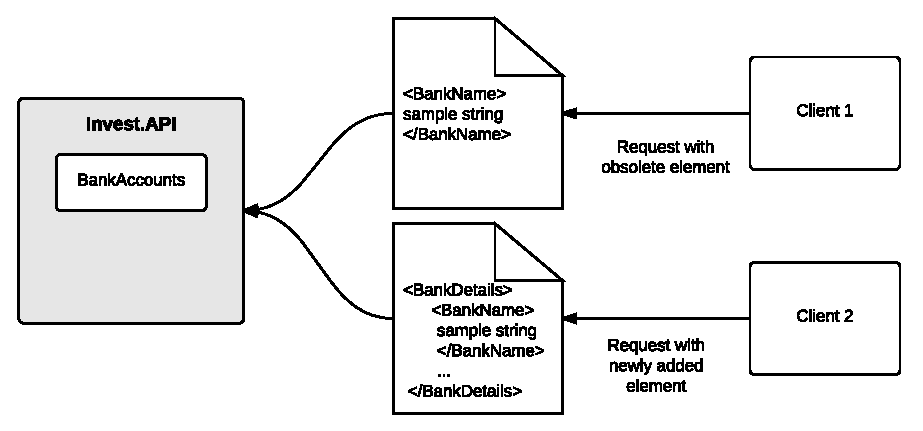
\includegraphics[width=12cm]{img/compatible-api-change.pdf}}
\caption{BankAccount service requests}
\label{fig:compatible-api-change}
\end{figure} 

It can happen that one of the clients have a specific change request which is out of the API functionality goals and moreover the change will be breaking. This change will be part of the new client-specific service (Figure \ref{fig:custom-service}). The service is than available just for this client. 

\begin{figure}[htp] \centering{
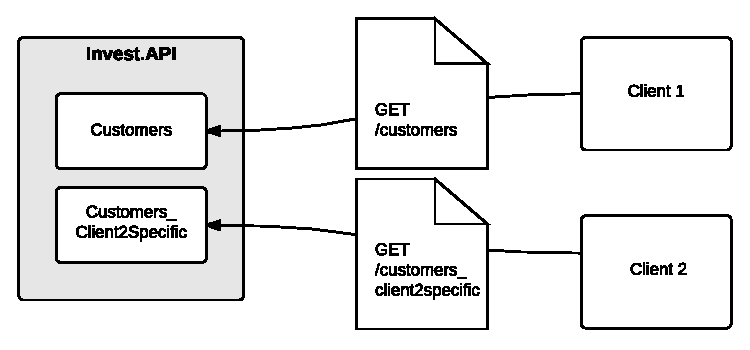
\includegraphics[width=10cm]{img/custom-service.pdf}}
\caption{Client-specific service}
\label{fig:custom-service}
\end{figure} 


At some point it occurs then there will be new version of API. All the duplications within a representation and the code are removed. The version of API is increased and it is created a new service documentation.

Versioning technique used by Invest s.r.o. is versioning on the level of service implementation. Every change which is done is made in code. There is just one version on API available for consumers. It is the one deployed on production environment. When a client ask for a change it is designed to be backward compatible.


\section{Summary}
Invest s.r.o doesn't utilize the service specific versioning approach and versions just an implementation. Although the version number is part of the URL there is no intention to create a new coexisting version accessible thanks to choice of particular endpoint address.
The Invest s.r.o. stands for versioning based on headers. Company's architecures believe it is a more RESTful approach. Implementation of headers for verisonig would reqire large amount of modifications on company side but also on client side. This decision would need a vast analysis. The integration of new approach would be a long term process. 







